% XPUShare — ICCIC 2026 submission
% LNCS format, double-blind
\documentclass[runningheads,a4paper]{llncs}

\usepackage[T1]{fontenc}
\usepackage{graphicx}

\graphicspath{{figures/}}
\usepackage{amsmath}
\usepackage{booktabs}
% \usepackage[hyphens]{url}
\usepackage{xurl}
\usepackage{microtype}
\usepackage{xcolor}
\newcommand{\doi}[1]{\url{https://doi.org/#1}}
\usepackage{listings}
\usepackage{placeins}
\usepackage{makecell}

\lstset{
  basicstyle=\ttfamily\small,
  breaklines=true,
  frame=single,
  xleftmargin=1em,
  xrightmargin=1em
}



\begin{document}

\title{XPUShare: A Containerized Cluster GPU Sharing Framework for Closed-Source CUDA-Like Heterogeneous Platforms}

\titlerunning{XPUShare: GPU Sharing for Closed-Source CUDA-Like Platforms}

% Double-blind submission — author info omitted
\author{Anonymous Author(s)}
\authorrunning{Anonymous}
\institute{}

\maketitle

\begin{abstract}
Cloud-native clusters increasingly require GPU sharing across training,
inference, and data-processing workloads. However, when clusters scale
from a single vendor to multi-vendor ``CUDA-like + closed-source runtime''
platforms, GPU sharing systems frequently fail during initial deployment:
device discovery schemas resist unification, container-visible device
binding semantics diverge across toolchains, and the API interception
boundary on the execution side may be unstable or bypassed entirely. To mitigate those difficulties, we propose XPUShare, a containerized cluster GPU sharing framework targeting
closed-source CUDA-like heterogeneous platforms. XPUShare decomposes the
sharing system into (i)~a cross-platform unified device view with minimal
telemetry, (ii)~an explicitly configurable and in-container verifiable
binding contract, and (iii)~a pluggable interception and arbitration
interface that treats boundary selection as a diagnosable deployment
decision with mutual-exclusion enforcement and safe rollback. We
implement an end-to-end prototype on a managed Kubernetes cluster with
Iluvatar BI-V150 GPUs and report evaluation results including
near-ideal weighted fairness ($J_w{\geq}0.995$) across five sharing
configurations, along with boundary reachability evidence, binding
consistency verification, and memory quota enforcement under closed-source
black-box conditions.

\keywords{GPU sharing \and containerized cluster \and CUDA-like \and
closed-source runtime \and cross-vendor \and user-space interception \and
verifiable contract}
\end{abstract}

%-----------------------------------------------------------------------
\section{Introduction}
%-----------------------------------------------------------------------
The rapid proliferation of GPUs in data centers has been driven by training and inference of deep neural networks (e.g., large language models). In practice, workloads rarely run in
isolation: throughput-oriented training and latency-sensitive inference
often share the same resource pool, while data preprocessing,
retrieval-augmented generation, and evaluation pipelines generate large
numbers of short-lived and bursty jobs. Under exclusive whole-card
allocation, GPU utilization is low, queue times are long, and resource
fragmentation is severe. Fine-grained sharing has therefore become a key
capability for cloud-native platforms seeking to improve GPU
efficiency. It has been explored in cluster scheduling systems (e.g.,
Gandiva and Salus)~\cite{gandiva,salus}, Kubernetes-integrated sharing
frameworks (e.g., KubeShare and Voda)~\cite{voda,kubeshare}, and
interference-aware fine-grained sharing for ML applications (e.g.,
Orion)~\cite{orion}; however, most prior systems assume a well-defined and
homogeneous GPU software stack and do not target deployment failures
induced by multi-vendor closed-source runtimes.

Existing GPU sharing systems have evolved along two main paths. The first
focuses on the \emph{control plane}: GPUs are exposed as first-class
schedulable resources via device plugins and extended schedulers, and
sharing is realized by mapping scheduling decisions to container-visible
device constraints~\cite{k8s-device-plugin,kubeshare}.
The second focuses on the \emph{execution plane}: in-process interception
of CUDA or CUDA-like API calls enables finer-grained time-slicing,
quota enforcement, and multi-tenant interference
control~\cite{gemini,cuda-interception}. Both approaches work well on a
single, well-understood platform. When clusters expand to multi-vendor
closed-source runtime environments, however, these systems tend to embed platform-specific assumptions into critical paths implicitly: discovery logic depends
on vendor-specific tool output fields, binding logic assumes a particular
environment variable name and value semantics, and execution control
assumes that a specific API boundary is always reachable. When migrating
to new platforms, these three assumptions may break, and
failures are difficult to identify.

Since Kubernetes is the de-facto substrate for accelerator management in
container clusters, these platform-specific assumptions are tightly
coupled with the Kubernetes device integration path. We summarize the
relevant ecosystem constraints (Device Plugin and CDI) and why they
matter to initial deployment on closed-source CUDA-like platforms in
Section~\ref{sec:background}.

Three fundamental engineering challenges are identified that account for the
majority of deployment failures on heterogeneous platforms: (i)~discovery
schema inconsistency across vendors (IDs/capacity/topology), (ii)~binding
semantic divergence across runtimes and toolchains (e.g., variable names and
index-vs-UUID semantics)~\cite{cdi,deepspark-toolkit},
and (iii)~execution-boundary uncertainty where interception may be
bypassed or unstable on closed-source runtimes~\cite{cuda-interception}.

This paper focuses on the system deployment and validation challenge on
closed-source CUDA-like platforms: how to build a migratable,
rollback-capable, and verifiable GPU sharing system without access to driver
or runtime source code. The goal is to stabilize the control path quickly
and convert boundary uncertainty into observable, configurable deployment
decisions. To this end, we propose a containerized cluster GPU sharing framework called XPUShare, organized around a staged
evidence chain: it first establishes a verifiable binding contract, then collects coverage signals for diagnosis, and finally makes an informed deployment decision---enforce or roll back.

Our contributions can be summarized as follows.
\begin{enumerate}
\item \textbf{Binding contract as a first-class artifact.} We make
explicit what variables to inject, what value semantics to use, and how to
verify the result inside the container---reducing cross-platform
misconfiguration risk.

\item \textbf{Configurable interception boundary with mutual-exclusion
enforcement.} We model execution-layer boundary selection as a deployment
decision, provide \texttt{profile/observe/enforce} three-stage modes, and guarantee
single-boundary enforcement and safe rollback in production.

\item \textbf{End-to-end prototype and evaluation.} We implement and
integrate XPUShare on a managed Kubernetes cluster with Iluvatar BI-V150
GPUs and report four categories of evidence: boundary reachability,
binding consistency, memory quota enforcement, and proportional sharing
with near-ideal weighted fairness ($J_w{\geq}0.995$).
\end{enumerate}

XPUShare separates framework invariants (minimal \texttt{DeviceView},
verifiable \texttt{BindingContract}, staged evidence chain,
mutual-exclusion + rollback) from replaceable mechanisms (discovery
provider, injection method, interception entry points, and enforcement
policy; cf.\ Section~\ref{sec:design}). This separation keeps the
control path stable while localizing vendor-specific adaptations to
swappable modules, reducing cross-vendor adaptation cost.

This paper is organized as follows.
In Section~\ref{sec:background} we review the background and formalize the
main engineering challenges. Section~\ref{sec:design} presents the design of XPUShare, whose prototype
implementation and platform integration are described in Section~\ref{sec:impl}. Section~\ref{sec:eval} presents our evaluation, with limitations discussed in Section~\ref{sec:discussion}. Section~\ref{sec:related} reviews related work and 
Section~\ref{sec:conclusion} concludes this paper.

%-----------------------------------------------------------------------
\section{Background and Challenges}
\label{sec:background}
%-----------------------------------------------------------------------

\subsection{Background and Terminology}

In Kubernetes-based clusters, GPU sharing is commonly
implemented by combining Device Plugin integrations with scheduler
extensions and vendor-specific visibility injection conventions, where
multi-vendor closed-source stacks often exhibit discovery and binding
divergence~\cite{cdi,k8s-device-plugin}. We target \emph{CUDA-like} accelerator platforms (CUDA-style runtime/driver
interfaces) under a \emph{black-box premise}: no driver/runtime source
access, relying on observable signals and rollback-capable boundaries to
reduce deployment cost. 

The term ``CUDA-like GPUs'' refers to graphics processors that adopt parallel computing architectures and programming models resembling NVIDIA's CUDA. They feature analogous hierarchical constructs---including threads (or work-items), warps (or equivalent SIMT execution units), thread blocks (or work groups), grids, and streaming multiprocessors—enabling massively parallel workloads. They typically support CUDA-compatible programming interfaces or provide straightforward migration paths from CUDA code. Vendors producing CUDA-like GPUs include Iluvatar CoreX, MetaX, Mthreads, etc.

\subsection{Three Key Engineering Challenges During Deployment}

\paragraph{Challenge~1: Discovery schema inconsistency.}
Different platforms expose different device identifiers and capacity
schemas; if such fields propagate into the scheduling core, migration
forces costly rewrites of scheduling and metering logic. For example,
NVIDIA exposes devices via \texttt{nvidia-smi} with UUID-based
identifiers, while Iluvatar CoreX uses \texttt{ixsmi} with index-based
enumeration and different capacity field names; a scheduler hard-coded
for one schema cannot discover devices on the other without source code modification.

\paragraph{Challenge~2: Binding convention instability and
unverifiability.}
Cloud-native systems commonly realize scheduling decisions by injecting a
visible-device set into the container environment, but variable names and
value semantics (index vs.\ UUID) diverge across
stacks~\cite{biren-plugin,cdi,deepspark-toolkit,metax-vllm,moorethreads-musa,paddleocr-metax}.
For instance, NVIDIA uses \texttt{NVIDIA\_VISIBLE\_DEVICES}, Iluvatar
uses \texttt{IX\_VISIBLE\_DEVICES}, and other vendors may use \texttt{X\_VISIBLE\_DEVICES} or alternative methods---each with potentially different index or UUID semantics. Failures often surface later as silent performance
anomalies rather than explicit errors.

\paragraph{Challenge~3: Execution boundary uncertainty.}
Interception-based sharing mechanisms rely on API interception at the
driver or runtime boundary to meter, rate-limit, and arbitrate GPU usage.
On closed-source runtimes, calls may bypass exported symbols via internal
fast paths, causing interception to trigger unreliably or not at
all~\cite{cuda-interception}; this silent failure undermines enforcement.

XPUShare addresses these challenges with explicit contracts and staged
deployment so that uncertainty becomes verifiable evidence for deployment
decisions.

%-----------------------------------------------------------------------
\section{XPUShare Framework Design}
\label{sec:design}
%-----------------------------------------------------------------------

\subsection{Design Principles}

XPUShare follows three principles: depend only on a minimal, stable device
view for control-plane decisions; treat binding and injection as explicit
configuration that is verifiable inside the container; and keep
execution-side enforcement optional, enabled only after profile/observe
signals confirm boundary reachability, with mutual-exclusion and rollback
retained in production.

\subsection{Overall Architecture and Data Flow}

Figure~\ref{fig:visio-chart} shows XPUShare's execution path and bypass-aware
interception workflow within a single compute node and container instance.
After an application thread issues a resource request or kernel launch via
a CUDA-like API, the call first enters the user-space interception layer
(XPUShare Shim). The shim performs a policy check and, via IPC, requests
authorization from the node-side management component; once authorized, it
forwards the call to the vendor's closed-source software stack
(runtime/driver), which ultimately drives the physical accelerator through
the kernel-mode driver. The red path in Fig.~\ref{fig:visio-chart} represents the
bypass that closed-source runtimes may introduce: critical operations may
skip the normal path and enter kernel mode directly, rendering interception
at ``one particular boundary'' unreachable or unstable.


\begin{figure}[t]
    \centering
    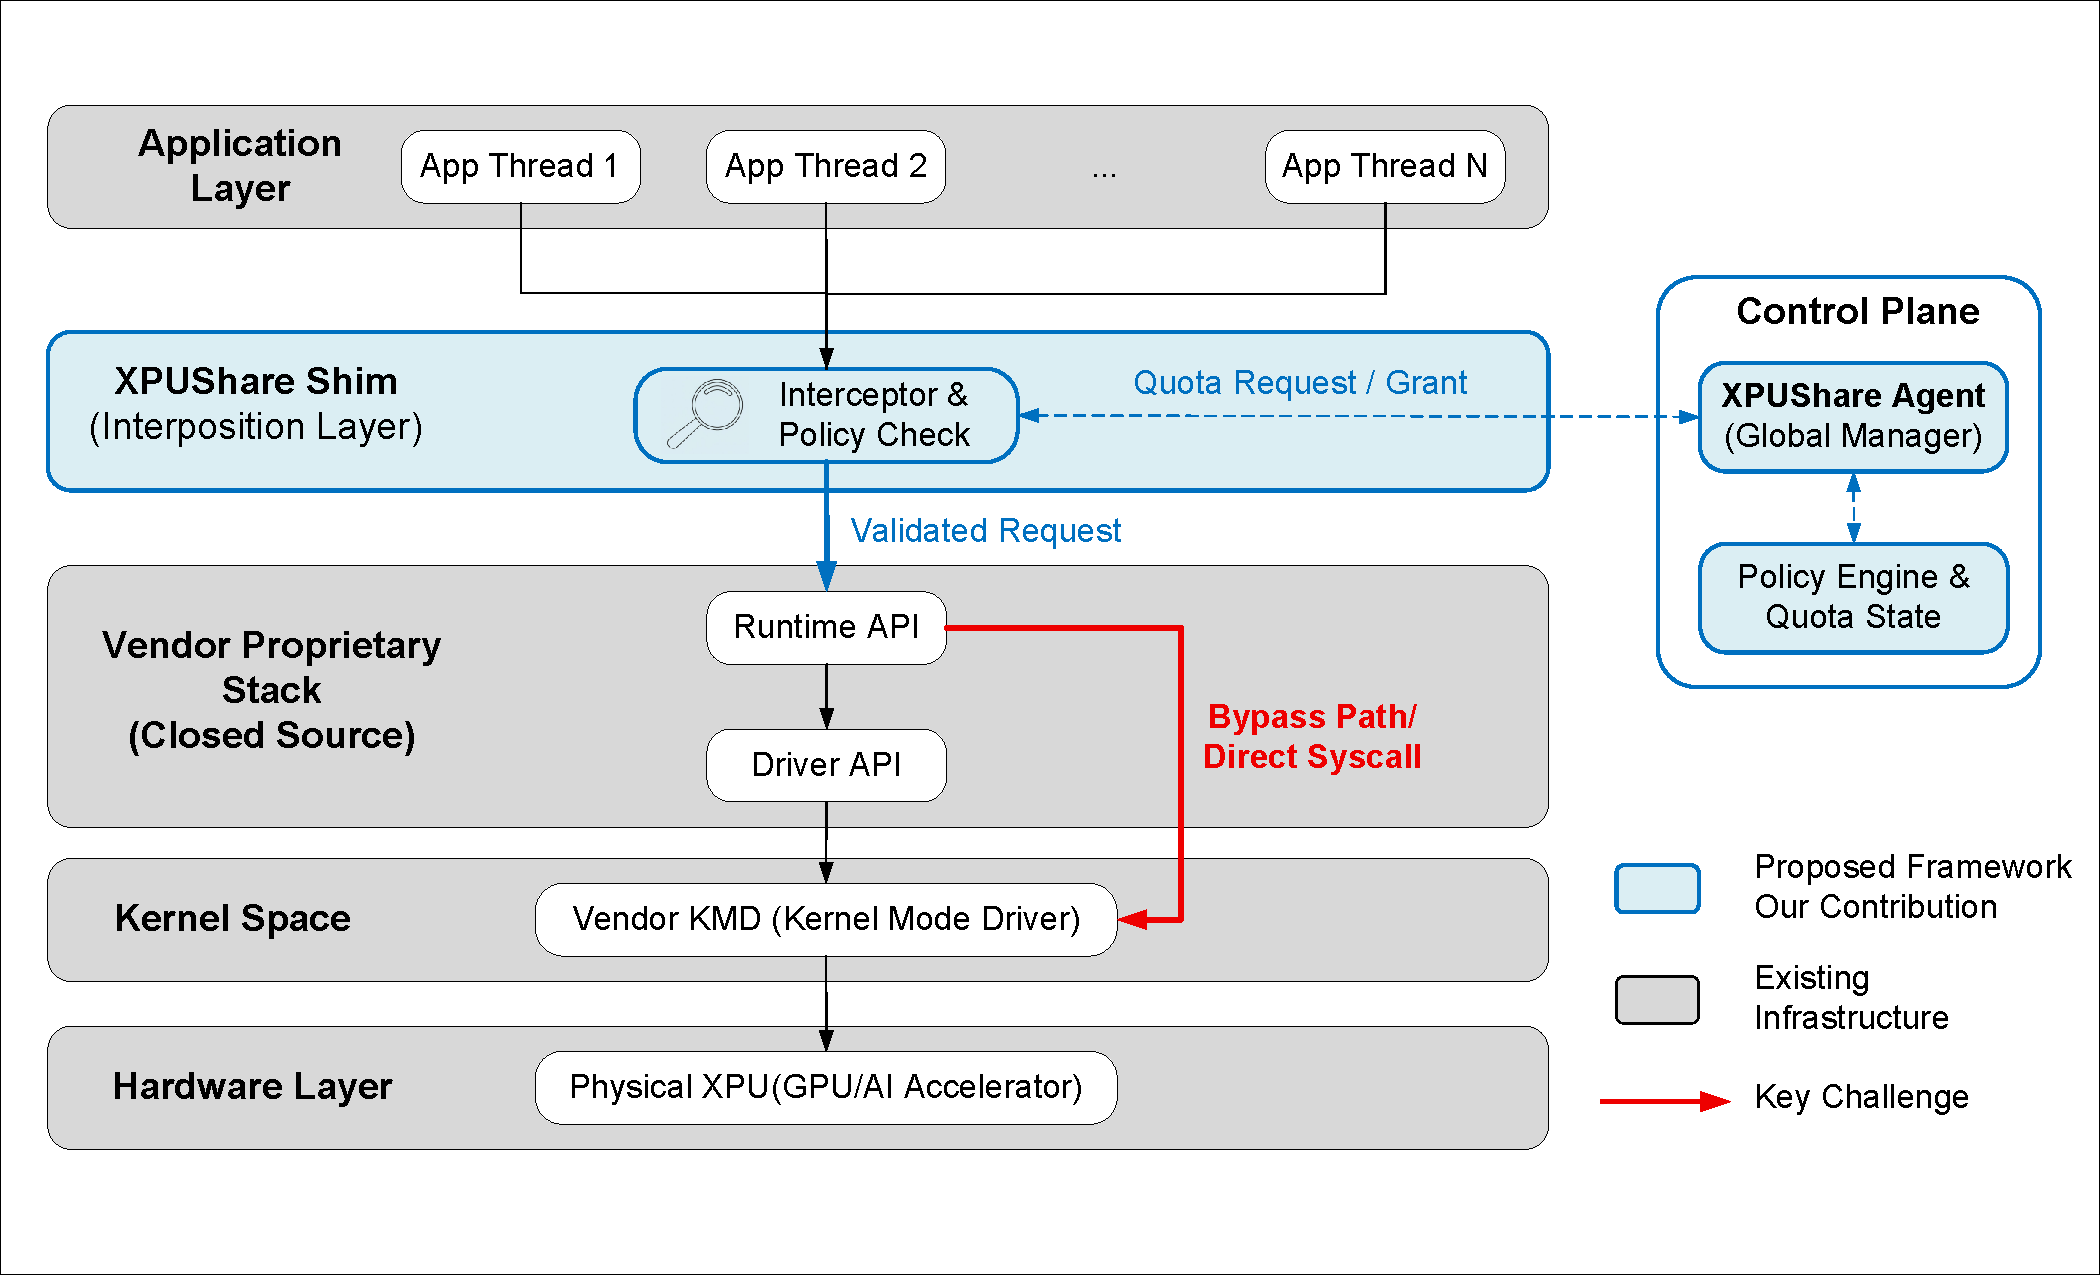
\includegraphics[width=1\linewidth]{1.pdf}
    \caption{XPUShare architecture and bypass-aware interception workflow.
  The red path illustrates the undocumented bypass that closed-source
  runtimes may introduce, bypassing the exported driver API boundary.}
    \label{fig:visio-chart}
\end{figure}

At the cluster level, XPUShare decomposes the sharing system into three
loosely coupled components: a node-side discovery collector that exports a minimal unified \texttt{DeviceView}; a control-plane scheduler/binder that maps selection to a verifiable \texttt{BindingContract}; and an optional execution-side
interception/arbitration layer that supports profile/observe/enforce modes
with mutual-exclusion enforcement and safe rollback.

XPUShare is a framework rather than a fixed mechanism: it mandates the
\texttt{DeviceView} schema, the \texttt{BindingContract} with in-container
verification, the evidence chain (contract $\to$ signal $\to$
profile/decision), and mutual-exclusion + rollback safety rules. Concrete
discovery providers, injection mechanisms, interception entry points, and
enforcement policies (quota, time-slicing, etc.) remain pluggable.

From an engineering perspective, the framework should not be deployed
``all features at once.'' Instead, deployment should proceed along a
verifiable evidence chain: it first closes the
discovery$\to$scheduling$\to$binding loop, then collects coverage signals
via profile/observe, and only then enables enforce with rollback retained.

\subsection{Key Abstractions: Device View and Binding Contract}

To prevent discovery schema differences from propagating into the
scheduling core, XPUShare defines a cross-platform unified device view
(\texttt{DeviceView}) as a minimal tuple:
\begin{equation}
D = (\mathit{uuid},\; \mathit{model},\; \mathit{memory\_bytes},\; \mathit{index})
\end{equation}
where \emph{uuid} is the stable device identifier (when available),
\emph{model} identifies the hardware SKU, \emph{memory\_bytes} records the
device's total memory capacity, and \emph{index} is the node-local device
index used by runtimes that only accept index-based binding. Optional
labels may be attached but are not hard dependencies for scheduling.

After a scheduling decision, the control plane generates a
\texttt{BindingContract} that maps the selected device set to a
container-visible constraint:
\begin{equation}
B = (\mathit{env\_names},\; \mathit{semantics},\; \mathit{visible\_set},\; \mathit{proof})
\end{equation}
where \emph{env\_names} lists the environment variables to inject,
\emph{semantics} $\in \{\texttt{uuid}, \texttt{index}\}$ specifies the
value format, \emph{visible\_set} records the selected devices, and
\emph{proof} is a minimal verification obligation: the device set derived
by reading the injected variables inside the container must match the
control-plane record.
Before enabling any execution enforcement, XPUShare requires a simple
presence/semantics/set-consistency gate; if any check fails, the operator
can reconfigure the enforcement layer to \texttt{none} (safe mode),
keeping the control path operational.

\subsection{Execution Layer: Pluggable Interception and Arbitration}

The execution layer provides a pluggable interception and arbitration
interface, making interception boundary selection configurable rather than hard-coded. The prototype supports three operating modes: \texttt{profile} emits count-only coverage signals, \texttt{observe} produces structured diagnostics, and \texttt{enforce} applies quota or time-slice decisions.

\noindent\textbf{Mutual-exclusion rule:} In production, a given workload
may be enforced by at most one boundary (e.g., runtime \emph{or} driver,
not both), preventing the same critical operation from being penalized
twice. When compatibility risk is unacceptable, the system must be able to
roll back to ``no enforcement'' safe mode, keeping the control-plane
scheduling and binding path operational.

%-----------------------------------------------------------------------
\section{Prototype Implementation and Platform Integration}
\label{sec:impl}
%-----------------------------------------------------------------------

This section describes the end-to-end prototype and highlights integration
points on a managed Kubernetes cluster with Iluvatar BI-V150 GPUs. A \emph{verifiable-path-first} approach is taken: the
discovery--scheduling--binding loop is closed correctly before any
execution-side capability is enabled.

\subsection{Implementation Overview}

The prototype consists of three pipelines. A per-node collector normalizes
platform tool output into \texttt{DeviceView} and exposes it via metrics.
The control plane schedules on \texttt{DeviceView} and materializes a
\texttt{BindingContract} by mutating Pod specs (injecting one or more
visible-device variables with explicit semantics and recording binding
evidence). Inside the container, an interception library is designed to hook the
CUDA-like API. When in \texttt{profile/observe} mode, this library emits coverage signals and
structured logs for diagnosis. When in \texttt{enforce} mode, it consults a node-side
arbitrator via IPC to apply quota/time-slice decisions under
mutual-exclusion and rollback rules.

The execution-side arbitrator employs a self-adaptive time-slice
mechanism: each client's kernel burst duration is predicted by an
exponentially weighted moving average (EMA) with a decaying maximum
envelope, and the granted quota is adjusted by an overuse feedback
factor that shrinks the quota for clients that consistently exceed their
allocation and slightly expands it for under-utilizing clients.
Scheduling priority among concurrent clients is determined by a
deficit-ratio comparator that normalizes each client's unmet demand by
its configured share weight, ensuring that proportional fairness
converges regardless of absolute weight magnitudes.

The collector uses a pluggable \texttt{Provider} interface to abstract
vendor-specific device discovery:

\begin{lstlisting}[language=Go,caption={Pluggable provider abstraction (simplified).}]
// Device maps to the DeviceView tuple (id, model, capacity).
type Device struct {
    UUID        string
    Model       string
    MemoryBytes uint64
    Index       int
}

// Provider abstracts vendor-specific device discovery.
type Provider interface {
    Name()    string
    Init()    error
    Devices() ([]Device, error)
}
\end{lstlisting}

\noindent The prototype includes providers for Iluvatar (\texttt{ixsmi}) as well as a generic command-line provider for
unsupported platforms. The active provider is selected at deployment time by the \texttt{XPU\_PROVIDER} environment variable.

\subsection{Platform Integration: Verifiable Binding Contract Injection}

In the managed Kubernetes environment, workload containers receive visible-device
constraints via environment variable injection performed by the control
plane. Because different toolchains may read multiple variable names
simultaneously, XPUShare explicitly lists all required variable names in
\texttt{BindingContract.\allowbreak env\_names} and writes them with unified
semantics (\texttt{uuid} or \texttt{index}). The in-container verification
procedure gates execution enforcement by checking variable presence, value
semantics, and set consistency against the control-plane record. If any check fails, the operator should keep the system in \texttt{observe/profile} mode or reconfigure to safe mode, preventing execution-side intervention from compounding an
already-broken binding.

\subsection{Platform Integration: Boundary Reachability Diagnosis}

The key risk on closed-source CUDA-like platforms is execution boundary
unreachability. In \texttt{profile/observe} mode, XPUShare emits \emph{boundary
coverage signals}: per-category call counts (kernel launch, memory
allocation, memory view/query, etc.) collected independently at the driver
boundary and the runtime boundary. The operator uses these signals to
configure the production enforce boundary (runtime/driver/none), and
the system enforces the mutual-exclusion rule at enforce time.
Section~\ref{sec:eval} quantifies this evidence and motivates a
configurable boundary: rather than hard-coding an assumption, XPUShare
externalizes the choice as a deployment decision backed by measurements.

\subsection{Experimental Environment}
\label{sec:env}

Experiments are conducted on a managed Kubernetes cluster, whose GPU
nodes are equipped with Iluvatar BI-V150 GPUs. To facilitate the
interpretability of experimental results, we use controlled microbenchmarks (e.g., repeated matrix
multiplication, stepped memory allocation) to isolate noise from data
loading, CPU affinity, and framework internals.
We use Iluvatar CoreX, a CUDA-like runtime/SDK, and \texttt{ixsmi} for
GPU management and version reporting.

\begin{table}[t]
\caption{Experimental environment parameters. The hardware, GPU runtime version, and selected software versions are listed. The remaining versions
are collected by standard commands (e.g., \texttt{containerd --version},
\texttt{ixsmi}, Iluvatar's GPU management utility).}
\label{tab:env}
\centering
\begin{tabular}{p{0.40\textwidth}p{0.53\textwidth}}
\toprule
\textbf{Parameter} & \textbf{Value} \\
\midrule
CPU (per node)              & 2$\times$ Phytium S5000C (aarch64), 128 physical cores total \\
Memory (per node)           & 1~TB (16$\times$64~GB) \\
GPU (per node)              & 8$\times$ Iluvatar BI-V150 cards (dual-die; 16 logical GPUs), 32~GB HBM2 per die, PCIe 4.0$\times$16 \\
Interconnect                & Broadcom PEX89104 PCIe switch (2 units, cascaded) \\
Cluster scale               & 1 GPU node; 8 BI-V150 cards (16 logical GPUs) \\
Kubernetes version    & Managed Kubernetes v1.23.17 \\
Node OS / Kernel            & KylinOS V10 (aarch64), Linux kernel 5.4+ \\
Container runtime (\texttt{containerd}) & containerd 1.7.15 \\
Iluvatar driver stack version  & IX-ML 4.3.0; Driver 4.3.6; CUDA-like Runtime 10.2 \\
Iluvatar CoreX version      & 4.3.6 \\
\bottomrule
\end{tabular}
\end{table}

%-----------------------------------------------------------------------
\section{Evaluation}
\label{sec:eval}
%-----------------------------------------------------------------------

We evaluate whether XPUShare can (i)~produce verifiable deployment evidence
under closed-source black-box conditions and (ii)~show minimal
execution-side effects using controlled microbenchmarks.

\subsection{E1: Execution Boundary Reachability (Coverage Signals)}
\label{sec:eval-e1}

\paragraph{Goal.}
Quantify whether interception at a given boundary (driver vs.\ runtime)
reliably reaches critical operation categories on a closed-source platform,
providing evidence for boundary selection.

\paragraph{Method.}
We run a fixed microbenchmark with coverage counting enabled at both
boundaries, parse the persisted hook log (\texttt{/xpushare/log/hook.log}
in our deployment), and aggregate symbols into operation categories. We
repeat the run three times and report per-category mean counts and CV.

\paragraph{Metrics.}
Per-category call counts (driver vs.\ runtime) and their coefficient of
variation (CV${}=\sigma/\mu$) across repeated runs.

\paragraph{Results.}
Across \textbf{N=3} repeated runs on BI-V150, the runtime-boundary hooks
consistently observed substantial kernel-launch activity (mean 9448.33,
CV 0.010) together with a small, stable number of memory-allocation events
(mean 6.00, CV 0.000) and memory view/query operations (mean 52.00, CV
0.000), while the corresponding driver-boundary counters remained zero
for all observed categories (Table~\ref{tab:e1} and Fig.~\ref{fig:e1-bar}). This indicates that
driver-boundary symbols can be bypassed in this closed-source stack, and
supports selecting the runtime boundary as the reachable enforcement
boundary in production.

\begin{table}[t]
\centering
\caption{E1 boundary reachability evidence (selected categories,
$N{=}3$ runs). In this table, driver boundary and runtime boundary are abbreviated as \textbf{drv} and \textbf{rt}, respectively.}

\label{tab:e1}
\begin{tabular}{p{0.26\textwidth}c@{\hspace{15pt}}c@{\hspace{15pt}}c@{\hspace{15pt}}c}
\toprule
\textbf{Category} & \textbf{drv mean} & \textbf{drv CV} & \textbf{rt mean} & \textbf{rt CV} \\
\midrule
kernel\_launch & 0.00 & 0.000 & 9448.33 & 0.010 \\
memory\_alloc  & 0.00 & 0.000 & 6.00 & 0.000 \\
memory\_view   & 0.00 & 0.000 & 52.00 & 0.000 \\
\bottomrule
\end{tabular}
\end{table}

\begin{figure}[t]
    \centering
    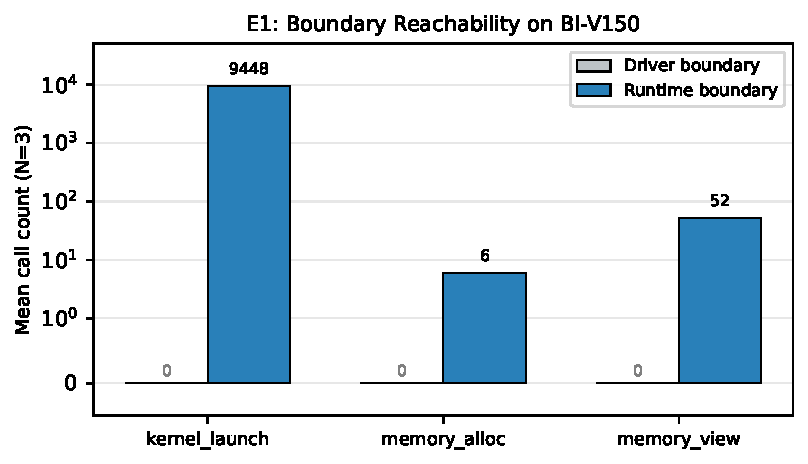
\includegraphics[width=0.85\linewidth]{fig-e1-boundary.pdf}
    \caption{E1 boundary reachability: driver-boundary counters remain zero
    while runtime-boundary hooks observe substantial activity across all
    operation categories (log scale, $N{=}3$).}
    \label{fig:e1-bar}
\end{figure}

\subsection{E2: Binding Consistency (Control-Plane Closed Loop)}
\label{sec:eval-e2}

\paragraph{Goal.}
Verify that control-plane binding decisions are faithfully reflected in the
container-visible device set, preventing silent ``scheduling correct,
binding broken'' failures.

\paragraph{Method.}
For each scheduled Pod, the control plane records the expected device set
in Pod annotations and injects visible-device environment variables. We
run a deployment checker that prints the injected visibility variables, and
we compare them against the scheduler-provided annotations to check
presence, index semantics, and set consistency.

\paragraph{Metrics.}
Binding verification pass rate, plus failure categorization (missing
variable / semantics mismatch / set mismatch).

\paragraph{Results.}
Across \textbf{N=3} independent deployment runs, the container-visible
binding was stable (Table~\ref{tab:e2}): \texttt{IX\_VISIBLE\_DEVICES}
consistently reported the same GPU index and matched the scheduler
annotation \texttt{sharedgpu/gpu\_index} in all runs, while
\texttt{sharedgpu/gpu\_uuid} was non-empty and stable across runs. The
environment snapshot also reported
\texttt{XPUSHARE\_ENFORCEMENT\_LAYER=runtime} and a non-empty
\texttt{LD\_PRELOAD}, indicating that runtime-boundary injection is active
on this stack.

\begin{table}[t]
\centering
\caption{E2 binding consistency evidence ($N{=}3$ independent deployment
runs). Each run re-creates the Pod from scratch; the checker compares the
injected \texttt{IX\_VISIBLE\_DEVICES} against the scheduler-written
annotation \texttt{sharedgpu/gpu\_index}.}
\label{tab:e2}
\begin{tabular}{c@{\hspace{5pt}}c@{\hspace{8pt}}c@{\hspace{8pt}}c@{\hspace{8pt}}c}
\toprule
\textbf{Run} & \textbf{\texttt{IX\_VISIBLE\_DEVICES}} & \textbf{\texttt{gpu\_index}} & \textbf{UUID present} & \textbf{Match} \\
\midrule
1 & 0 & 0 & Yes & PASS \\
2 & 0 & 0 & Yes & PASS \\
3 & 0 & 0 & Yes & PASS \\
\bottomrule
\end{tabular}
\end{table}

\subsection{E3: Memory View Consistency and Quota Enforcement}
\label{sec:eval-e3}

\paragraph{Goal.}
Confirm that memory quota enforcement changes the in-container observable
memory view and yields a predictable failure point for over-quota
allocations.

\paragraph{Method.}
We configure a memory quota via Pod metadata and run a stepped allocator
that increases allocation size; we log \texttt{mem\_get\_info} and record
the first allocation failure to compare against the configured quota. To
	test generality, we repeat the procedure under three quota settings
	(2\,GiB, 4\,GiB, and 8\,GiB) on the same physical GPU.

\paragraph{Metrics.}
Consistency between reported total memory and configured quota; first
failure point, measured in absolute bytes and as a ratio to the quota;
and failure explainability, including error type and logs.

\paragraph{Results.}
Across all three quota settings (2, 4, and 8\,GiB), the in-container
	memory queries reported a total matching the configured quota (instead of
	the physical 32\,GB device capacity), indicating a quota-consistent memory
	view (Table~\ref{tab:e3}). In each case, a moderate allocation succeeded
	and was reclaimed, while an over-quota request constructed as
	(\emph{reported free} + 100\,MiB) failed with \texttt{OutOfMemoryError}.
	The failure-to-quota ratio decreases with larger quotas
	(1.049$\times$ at 2\,GiB, 1.024$\times$ at 4\,GiB, 1.012$\times$ at
	8\,GiB) because the fixed 100\,MiB over-allocation becomes a smaller
	fraction of the total, confirming that the enforcement boundary tracks the
	configured quota rather than a fixed offset.

\begin{table}[!htbp]
\centering
\small
\caption{E3 memory view consistency and quota enforcement evidence
(BI-V150, 32\,GB HBM2 per die). Over-alloc = \emph{reported free} +
100\,MiB; ratio = over-alloc point\,/\,quota.}
\label{tab:e3}
\begin{tabular}{@{}c@{\hspace{12pt}}c@{\hspace{12pt}}c@{\hspace{12pt}}c@{\hspace{15pt}}c@{}}
\toprule
\textbf{\shortstack{Quota\\(GiB)}} & \textbf{\shortstack{Rpt.\ total\\(GiB)}} & \textbf{\shortstack{Over-alloc\\(MiB)}} & \textbf{Ratio} & \textbf{Err} \\
\midrule
2.0 & 2.0 & 100 & 1.049$\times$ & \texttt{OutOfMemoryError} \\
4.0 & 4.0 & 100 & 1.024$\times$ & \texttt{OutOfMemoryError} \\
8.0 & 8.0 & 100 & 1.012$\times$ & \texttt{OutOfMemoryError} \\
\bottomrule
\end{tabular}
\normalsize
\end{table}

\subsection{E4: Two-Pod Proportional Sharing (Execution-Side Evidence)}
\label{sec:eval-e4}

\paragraph{Goal.}
Show that execution-side enforcement can \emph{differentiate} two Pods on
the same physical GPU according to configured share weights, improving
weighted proportionality beyond a control-plane-only baseline.

\paragraph{Method.}
Two Pods run the same matrix-multiplication microbenchmark ($2048\times2048$ FP16 \texttt{matmul}, 60\,s) concurrently on one physical GPU. We test five
weight configurations spanning equal shares ($w_A{=}w_B$) and unequal shares
with target ratios from 1.0 to 3.0. Each configuration is averaged over
$N{=}5$ rounds. We compare (i)~a control-plane-only baseline
(scheduling and binding active, but no execution-side enforcement) and (ii)~XPUShare
with execution-side enforcement enabled, where the arbitrator uses
EMA-based burst prediction, overuse-aware quota adjustment, and
deficit-ratio priority scheduling. A single-Pod $w{=}1.0$ run serves as
the full-GPU throughput reference.

\paragraph{Metrics.}
We report per-Pod throughput (iterations/s), throughput ratio $x_B/x_A$
(ideal target $w_B/w_A$), and a weighted Jain fairness index computed over
weight-normalized throughput $y_i = x_i/w_i$ (ideal $J_w{=}1$):
\begin{equation}
J_w = \frac{\left(\sum_i y_i\right)^2}{n \sum_i y_i^2}, \quad y_i = \frac{x_i}{w_i}.
\end{equation}

\paragraph{Results.}
Table~\ref{tab:e4} reports the baseline and five XPUShare configurations, together with resultant Jain fairness indices.
Without execution-side enforcement, the baseline yields near-equal
throughput ($x_B/x_A{=}1.00$, $J_w{=}0.900$), confirming that the control
plane alone cannot differentiate shares.
This value is below~1 despite equal throughput because the weighted index
normalizes by share weight: $y_A{=}x_A/w_A$ and $y_B{=}x_B/w_B$ diverge
when $w_A{\neq}w_B$, penalizing the failure to allocate proportionally.
With enforcement enabled, the
throughput ratio consistently tracks the weight ratio across all five
configurations: $x_B/x_A{=}2.01$ for target~2.0, 2.59 for target~3.0,
1.32 for target~1.5, and close to~1.0 for equal-share settings. The
weighted Jain index $J_w$ ranges from 0.995 to 1.000 (mean 0.998),
indicating near-ideal proportional fairness (Fig.~\ref{fig:e4-ratio}).
The ratio deviation from target is 7--10\% for 1{:}1,
	0.5\% for 1{:}2, and 13.7\% for 1{:}3. This is consistent with a
	throughput floor effect: GPU kernels are non-preemptive, so the
	low-weight Pod completes at least one kernel per scheduling cycle
	regardless of its share, and the fixed IPC overhead of the shim
	consumes a larger fraction of the low-weight Pod's time budget.
	Both factors compress the achievable ratio at extreme weight
	disparities. The overuse-aware quota adjustment partially
	compensates for this effect by reducing the granted time-slice for
	clients that consistently exceed their allocation, but the
	non-preemptive kernel granularity remains the fundamental limiting
	factor.

\begin{table}[t]
\centering
\caption{E4 proportional sharing evidence ($N{=}5$ rounds per configuration;
single-Pod $w{=}1.0$ reference: 4189.80\,iters/s).}
\label{tab:e4}
\begin{tabular}{c@{\hspace{10pt}}c@{\hspace{10pt}}c@{\hspace{10pt}}c@{\hspace{10pt}}c@{\hspace{10pt}}c@{\hspace{10pt}}c}
\toprule
\textbf{Configuration} & $w_A$ & $w_B$ & $x_A$ & $x_B$ & $x_B/x_A$ & $J_w$ \\
\midrule
Baseline (no enforce) & 0.2 & 0.4 & 2093.08 & 2092.25 & 1.00 & 0.900 \\
\midrule
XPUShare (equal 0.2)  & 0.2 & 0.2 & 1020.69 &  953.80 & 0.93 & 0.999 \\
XPUShare (equal 0.3)  & 0.3 & 0.3 & 1393.65 & 1539.74 & 1.10 & 0.998 \\
XPUShare (2:3)        & 0.2 & 0.3 &  982.05 & 1298.04 & 1.32 & 0.996 \\
XPUShare (1:2)        & 0.2 & 0.4 &  940.06 & 1893.94 & 2.01 & 1.000 \\
XPUShare (1:3)        & 0.1 & 0.3 &  511.41 & 1325.05 & 2.59 & 0.995 \\
\bottomrule
\end{tabular}
\end{table}

A scheduling sanity check further confirms correctness: when two Pods
request $w_A{=}0.4$ and $w_B{=}0.8$ (total exceeding 1.0), the scheduler
places them on separate physical GPUs, as expected.

\begin{figure}[t]
    \centering
    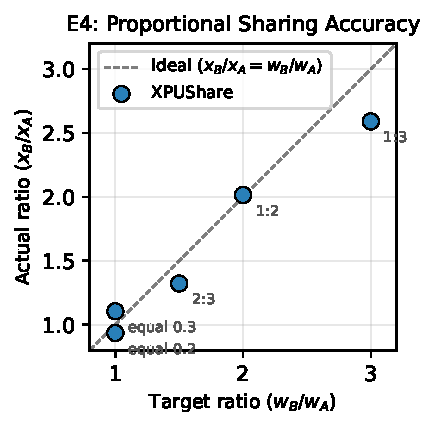
\includegraphics[width=0.5\linewidth]{fig-e4-ratio.pdf}
    \caption{E4 target vs.\ actual throughput ratio across five sharing
    configurations. Points near the dashed ideal line indicate accurate
    proportional enforcement; the 1:3 configuration shows a 13.7\%
    deviation at the highest target ratio.}
    \label{fig:e4-ratio}
\end{figure}

%-----------------------------------------------------------------------
\section{Discussion}
\label{sec:discussion}
%-----------------------------------------------------------------------

\paragraph{Limitations and interpretation.}
Our evaluation targets a minimal evidence chain on a single GPU node using
controlled microbenchmarks. E4 demonstrates near-ideal weighted fairness
($J_w{\geq}0.995$) across five weight configurations, but the evaluation
scope remains limited: real training and inference workloads exhibit more
complex memory access patterns and kernel scheduling behavior that may
reduce fairness.
	In E4, the 1{:}3 configuration exhibits a 13.7\% deviation from the
	target ratio. The self-adaptive quota mechanism---EMA-based burst
	prediction with overuse feedback and deficit-ratio priority---converges
	well for moderate weight ratios (1{:}1 to 1{:}2) but faces a
	fundamental floor at extreme disparities: GPU kernels are
	non-preemptive, so the low-weight client executes at least one kernel
	per scheduling cycle regardless of its configured share, and the
	IPC-based arbitration overhead consumes a proportionally larger
	fraction of the low-weight client's time budget. Reducing this gap
	would require finer-grained preemption support, which is unavailable
	on the current closed-source stack.
	Multi-node scaling and longer-term stability analysis are
left for future work.

\paragraph{Interception boundary selection.}
XPUShare does not prescribe which boundary to use. The configurable
boundary design and mutual-exclusion enforcement rule apply regardless of
which boundary is selected. Platform integrators should stabilize the
control path first, then use profile/observe signals to select the
boundary, and only then enable enforce with rollback retained. The
diagnostic mechanism itself is not the only valid approach---any
method that externalizes boundary uncertainty as reproducible evidence
is acceptable.

\paragraph{Security and generality scope.}
This work does not target adversarial multi-tenant isolation; if tenants
are untrusted, stronger isolation mechanisms and threat-model-driven
analysis are required~\cite{guardian}. XPUShare is complementary to broader
XPU scheduling abstractions (e.g., XSched)~\cite{xsched}: we focus on
deployment evidence and verifiable integration surfaces under closed-source
runtime uncertainty.

%-----------------------------------------------------------------------
\section{Related Work}
\label{sec:related}
%-----------------------------------------------------------------------

Kubernetes exposes accelerators as schedulable resources via device plugins
and related ecosystem interfaces~\cite{gpushare-extender,voda,k8s-device-plugin,nvidia-device-plugin,kubeshare},
but cross-vendor deployment remains fragile when discovery schemas and
container-visible binding conventions diverge. Execution-side designs use
in-process interception and scheduling to implement time-slicing, quotas,
and interference control~\cite{gemini,cuda-interception,orion}, which XPUShare complements by treating interception boundary reachability as an
explicit, diagnosable deployment decision backed by coverage evidence.

\paragraph{Cluster-level GPU sharing.}
Gandiva~\cite{gandiva} introduces introspective scheduling for deep
learning clusters but assumes a homogeneous NVIDIA stack.
Salus~\cite{salus} provides fine-grained GPU sharing primitives at the
framework level; it does not address container-level binding or
cross-vendor discovery. KubeShare~\cite{kubeshare} and
Voda~\cite{voda} integrate GPU sharing into Kubernetes via device plugins
and scheduler extensions, but neither provides a verifiable binding
contract or handles closed-source runtime divergence. 
XPUShare adds cross-platform abstractions and
verifiable binding contracts to the device-plugin scheduling approach.

\paragraph{Execution-side interception and isolation.}
Gemini~\cite{gemini} implements multi-tenant GPU sharing based on kernel
burst estimation via CUDA API interception; it assumes a stable,
reachable interception boundary and uses a monotone-queue predictor with
overlap-splitting usage accounting. XPUShare replaces the predictor with
an EMA-plus-decaying-maximum estimator and introduces overuse-aware quota
feedback and deficit-ratio priority scheduling, improving proportional
convergence under heterogeneous weight configurations. Tsiachris et
al.~\cite{cuda-interception} study fine-grained CUDA call interception
for GPU virtualization but do not address boundary bypass on closed-source
stacks. Guardian~\cite{guardian} analyzes protection boundaries in
multi-tenant GPU sharing from a security perspective. Complementary to these mechanisms, XPUShare could serve as a framework for selecting and
validating which boundary to use when the runtime is a black box.

\paragraph{GPU multiplexing and cross-XPU scheduling.}
NVIDIA MIG~\cite{nvidia-mig} and Chimera~\cite{chimera} provide
hardware-level or compiler-level GPU multiplexing for concurrent
workloads; both are tied to specific hardware. XSched~\cite{xsched}
proposes a unified preemptive scheduling abstraction across various XPUs;
XPUShare is complementary, focusing on container-cluster deployment and
verifiable contracts under closed-source uncertainty rather than
cross-XPU scheduling abstractions.

%-----------------------------------------------------------------------
\section{Conclusion}
\label{sec:conclusion}
%-----------------------------------------------------------------------
	
We presented XPUShare, a containerized cluster GPU sharing framework for
closed-source CUDA-like heterogeneous platforms. XPUShare decomposes GPU sharing into a unified device view with minimal telemetry, an
explicitly configurable and verifiable binding contract, and a pluggable
user-space execution enforcement layer with self-adaptive time-slice
arbitration. Interception boundary selection is
modeled as a diagnosable, configurable deployment decision subject to
mutual-exclusion enforcement and safe rollback. We implemented an
end-to-end prototype on a managed Kubernetes cluster with Iluvatar BI-V150
GPUs and reported four categories of evaluation evidence: 
boundary reachability, binding consistency, enforcement of memory quota, and
proportional sharing with near-ideal weighted fairness
($J_w{\geq}0.995$) across five sharing configurations.
Future work will extend the evaluation to more platforms, more complex
training and inference workloads, multi-node scaling, and longer-term
stability analysis.

%-----------------------------------------------------------------------
% Bibliography
%-----------------------------------------------------------------------
\bibliographystyle{splncs04}
\bibliography{Ref}          

\end{document}
